
\documentclass[border=4pt]{standalone}
\usepackage[utf8]{inputenc}
\usepackage[T1]{fontenc}
\usepackage{amsmath,amssymb,xcolor}
\usepackage{tikz}
\usetikzlibrary{arrows.meta,shapes.misc}
\renewcommand{\familydefault}{\sfdefault}
\definecolor{vbleu}{HTML}{1C5FD6}
\definecolor{orange}{HTML}{E8590C}
\definecolor{vert}{HTML}{2F9E44}
\definecolor{gris}{HTML}{495057}
\definecolor{violet}{HTML}{7048E8}
\tikzset{
  vec/.style={->,very thick,>={Stealth[length=2.4mm]}},
  ref/.style={orange,thick,dashed},
  par/.style={vert,thick,dashed},
  sec/.style={gris,thick,dashed},
  ptcross/.style={cross out,draw,thick,minimum size=1.6mm,inner sep=0pt},
}
\begin{document}
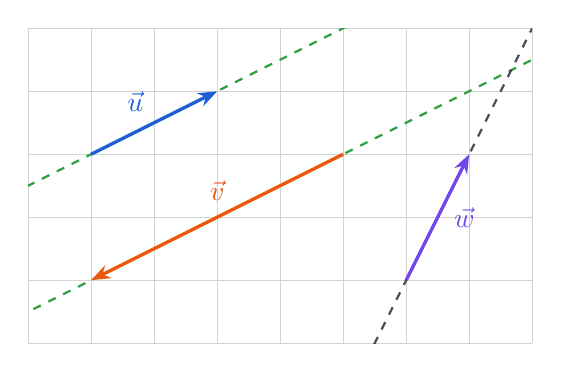
\begin{tikzpicture}[x=0.5cm,y=0.5cm]
\begin{scope}[x=0.8cm,y=0.8cm]
\draw[gray!35,thin,step=0.8cm] (0,0) grid (8,5);
\begin{scope}\clip (0,0) rectangle (8,5);
\draw[par] (-79,-37) -- (81,43);
\draw[par] (165,83) -- (-155,-77);
\draw[sec] (-34,-79) -- (46,81);
\end{scope}
\draw[vec,vbleu] (1,3) -- (3,4) node[midway,above left] {$\vec{u}$};
\draw[vec,orange] (5,3) -- (1,1) node[midway,above=2pt] {$\vec{v}$};
\draw[vec,violet] (6,1) -- (7,3) node[midway,right=2pt] {$\vec{w}$};
\end{scope}

\end{tikzpicture}
\end{document}
